\documentclass{oci}
\usepackage[utf8]{inputenc}
\usepackage{graphicx}
\usepackage{lipsum}

\title{Dados para Sótanos y Lagartos}

\begin{document}
\begin{problemDescription}
  Hernán es fanático de los juegos de rol.
  En particular, su juego favorito siempre ha sido Sótanos y Lagartos.
  Cómo en muchos juego de rol, para jugar Sótanos y Lagartos se
  necesita un conjunto especial de dados.
  Estos dados son especiales porque además del tradicional
  dado de 6 caras también hay dados con una mayor cantidad de caras.
  La siguiente imagen muestra un conjunto básico con dados de
  6, 8, 12 y 20 caras.
  \begin{center}
    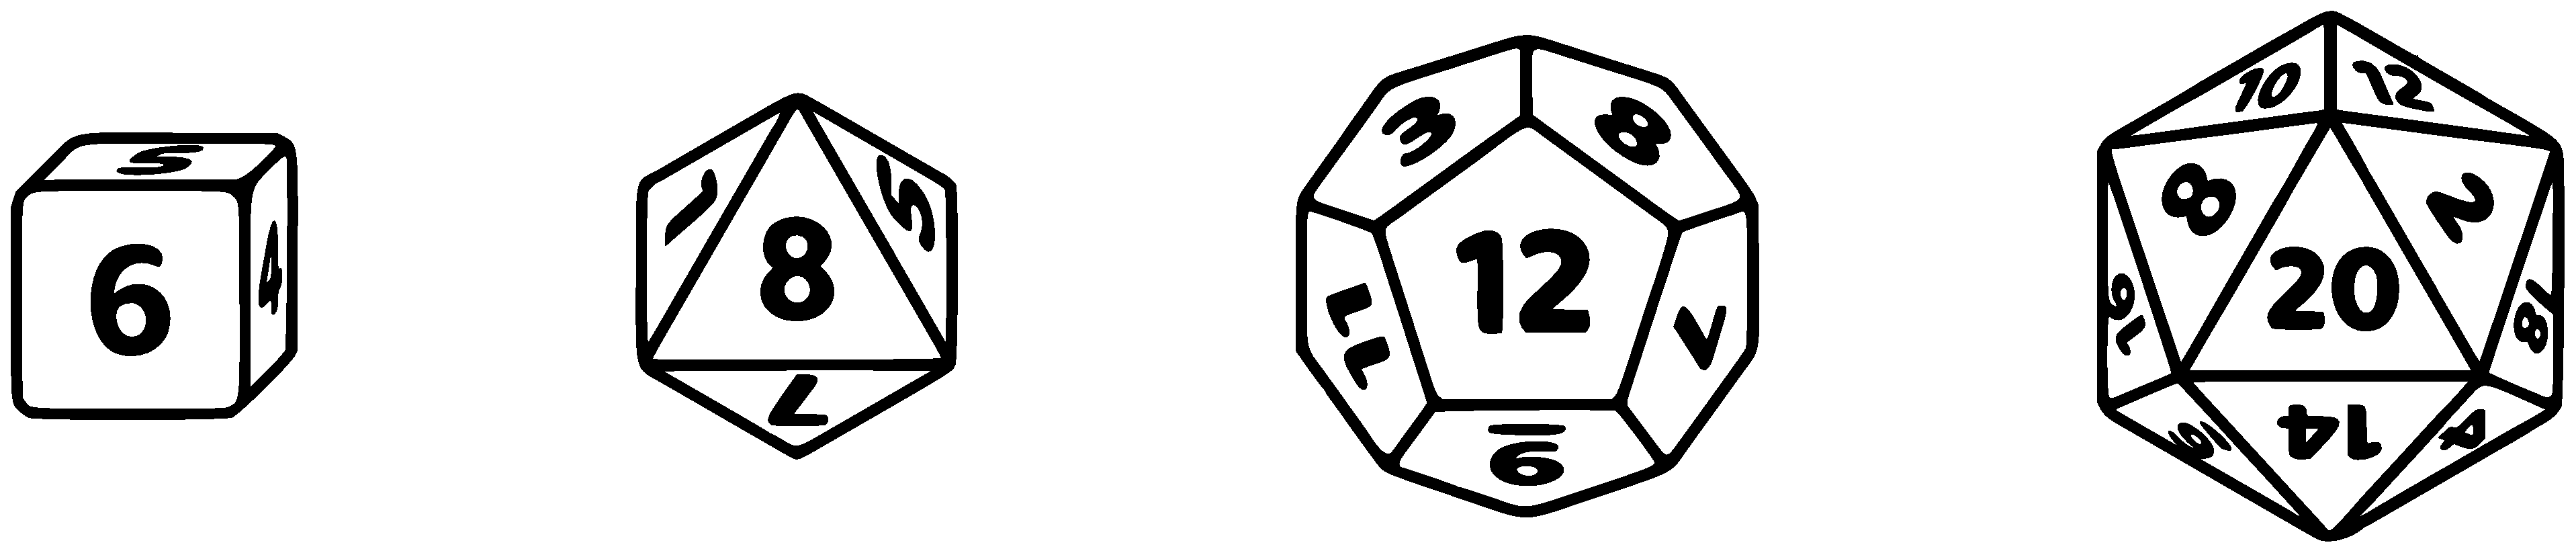
\includegraphics[scale=0.2]{horizontal-sin4}
  \end{center}

  Luego de años ganando experiencia, Hernán ha llegado al
  punto donde su conjunto básico ya no le es suficiente para
  las campañas más avanzadas y necesita dados con aún más caras.
  Tras días mirando en el mercado aún no ha podido encontrado
  un diseño que lo satisfaga así que decidió hacer sus propios
  dados.

  Hernán quiere que sus dados sigan la norma internacional
  de Sótanos y Dragones.
  Para seguir la norma, un dado de $n$ caras debe cumplir las
  siguientes dos propiedades:
  \begin{enumerate}
    \item Cada cara debe tener un valor diferente entre $1$ y $n$.
    \item La suma de los valores de dos caras opuestas debe ser siempre $n+1$.
  \end{enumerate}
  Por ejemplo, en el tradicional dado de 6 caras, cada cara está numerada
  con un valor diferente entre $1$ y $6$, y el 1 está opuesto al 6,
  el 2 al 5 y el 3 al 4.

  Dado un dado de $n$ caras y un valor $v$ en una de sus caras, llamamos
  complemento al valor que sumado a $v$ da $n+1$.
  Por ejemplo, en un dado de 6 caras el complemento de 1 es 6 (y viceversa)
  el complemento de 2 es 5 (y viceversa) y el complemento de 3 es 4 (y viceversa).

  Hernán ya ha escogido los valores para la mitad
  de las caras de un dado y ahora se pregunta si es posible completar
  la otra mitad cumpliendo con la norma internacional de
  Sótanos y Dragones.
  Específicamente, dada la lista de valores para la mitad de las caras, un
  dado puede completarse si para cada valor en la lista, su complemento no se
  encuentra en la lista.
  ?`Podrías ayudarlo?
\end{problemDescription}

\begin{inputDescription}
  La primera línea de la entrada contiene un entero $n$ ($2 \leq n \leq 10^6$)
  correspondiente a la cantidad de caras en el dado.
  Se garantiza que $n$ es par.

  La siguiente línea contiene $n/2$ enteros distintos entre $1$ y $n$ indicando
  el valor en las caras de la primera mitad del dado.
\end{inputDescription}

\begin{outputDescription}
  En caso de ser posible completar el dado de acuerdo a las restricciones del enunciado,
  la salida debe decir \texttt{SI}. En caso contrario, la salida debe decir \texttt{NO}.
\end{outputDescription}

\begin{scoreDescription}
  \subtask{50} Se probarán varios casos de prueba donde $n \leq 500$.
  \subtask{50} Se probarán varios casos de prueba sin restricciones adicionales.
\end{scoreDescription}

\begin{sampleDescription}
\sampleIO{sample-1}
\sampleIO{sample-2}
\end{sampleDescription}

\end{document}
